\chapter{Grundlagen}

\label{cha_basics}

\todo{Nach Einleitung nochmal umschreiben}

Dieses Kapitel widmet sich den Grundlagen der in dieser Arbeit verwendeten Konzepte, Verfahren und Systeme. Zu Beginn werden für den Verlauf der Arbeit notwendige Definitionen gegeben. Anschließend werden die juristischen Hintergründe des Arbeitnehmerdatenschutzes erläutert, die den rechtlichen Rahmen für das Thema dieser Arbeit bilden. 

Es folgen Erläuterungen zu SIEM-Systemen, in die - wie bereits in der Einleitung erläutert - die prototypische Umsetzung der datenschutzfreundlichen Speicherung erfolgen soll, sowie zu den zu verwendenden Datenschutztechniken Pseudonymisierung, kryptographische Schwellwertschemata und Searchable Encryption.

\section{Definitionen und Notationen}

\label{sec_basics_definitions}

%- Insider-Angriff
%- Datenarten
%- Syslog?

\subsection{Mathematische Notationen}

\(p,q\)

\(\mathbb{Z}_p\)

\(\mathbb{Z}_p^*\)

\section{Arbeitnehmerdatenschutz}

\label{sec_basics_employee_privacy}

\todo{Gesetzestexte als "`Quellen"` in Fußnoten?}

Der Begriff des Arbeitnehmerdatenschutzes\footnote{
  In manchen Veröffentlichungen wird der Arbeitnehmerdatenschutz auch als Mitarbeiterdatenschutz, Beschäftigtendatenschutz, Personaldatenschutz oder Betriebsdatenschutz bezeichnet.
}
beschreibt die Rechte von Arbeitnehmern im Beschäftigungsverhältnis im Bezug auf den Umgang mit personenbezogenen Daten. In diesem Abschnitt soll ein kompakter Überblick über aktuell geltende und in nächster Zeit in Kraft tretende gesetzliche Regelungen im Bezug hierauf gegeben werden, wobei der Fokus auf zum Thema der Arbeit passenden Regelungen liegt.

Zu Beginn soll kurz auf das Recht auf informationelle Selbstbestimmung eingegangen werden, das die Grundlage für alle folgenden Betrachtungen zum Arbeitnehmerdatenschutz bildet.

\subsection{Das Recht auf informationelle Selbstbestimmung}

Im sogenannten Volkszählungsurteil aus dem Jahr 1983 wurde das Recht auf informationelle Selbstbestimmung als Grundrecht anerkannt \cite{TODO}. 
Es handelt sich um eine Ausprägung des allgemeinen Persönlichkeitsrechts\footnote{
  Das allgemeine Persönlichkeitsrecht beschreibt den Schutz der Persönlichkeit einer Person vor Eingriffen in ihren Lebens- und Freiheitsbereich.
} nach Artikel 2, Absatz 1 in Verbindung mit Artikel 1, Absatz 1 des Grundgesetzes. Es beschreibt das Recht des Einzelnen, selber über den Umgang mit seinen personenbezogenen Daten entscheiden zu können. 

%    \todo{Nötig?}
%    \begin{quotation}
%    Die Würde des Menschen ist unantastbar. Sie zu achten und zu schützen ist Verpflichtung aller staatlichen Gewalt.
%    
%    \textit{-- Artikel 1, Absatz 1, GG}
%    
%    Jeder hat das Recht auf die freie Entfaltung seiner Persönlichkeit, soweit er nicht die Rechte anderer verletzt und nicht gegen die verfassungsmäßige Ordnung oder das Sittengesetz verstößt. 
%        
%    \textit{-- Artikel 2, Absatz 1, GG} 
%    \end{quotation}
    
Mit dem vermehrten Aufkommen automatisierter Datenverarbeitung stellten die Richter des Bundesverfassungsgerichts damals die besondere Schutzbedürftigkeit der Selbstbestimmung des Einzelnen im Bezug auf die Offenbarung von Lebenssachverhalten heraus. Sie betonten die Notwendigkeit dieser Selbstbestimmung als Voraussetzung für eine freie Entfaltung der Persönlichkeit und auch für die Ausübung bestimmter Grundrechte wie der Versammlungsfreiheit. Damit sei das Recht auf informationelle Selbstbestimmung auch \glqq eine elementare Funktionsbedingung eines auf Handlungs- und Mitwirkungsfähigkeit seiner Bürger begründeten freiheitlichen demokratischen Gemeinwesens\grqq{} \cite{TODO} .
    
Einschränkungen dieses Rechts sind dem Urteil nach möglich, jedoch in Gesetzen festzuhalten. Hierbei müssen das Geheimhaltungsinteresse des Betroffenen und das öffentliche Informationsinteresse verarbeitender Stellen gegeneinander abgewogen werden.

Auch wenn sich das Urteil des Bundesverfassungsgerichts nur auf die Rechte des Betroffenen gegenüber staatlichen Akteuren bezieht, so bildet die Intention des Rechts auf informationelle Selbstbestimmung doch die Grundlage für das heutige Bundesdatenschutzgesetz und auch die Datenschutzgrundverordnung der EU, die auch für nicht-staatliche Akteure Gültigkeit besitzen.

Zusätzlich findet sich das Recht auf informationelle Selbstbestimmung auch in der Grundrechtecharta der EU: \glqq Jede Person hat das Recht auf Schutz der sie betreffenden personenbezogenen Daten.\grqq{}\todo{Quelle}\footnote{
  Artikel 8, Absatz 1
}

\subsection{Datenschutz im Beschäftigungsverhältnis}

Eine besondere Situtation ergibt sich im Unternehmenskontext. Hier muss das Recht des Arbeitnehmers auf informationelle Selbstbestimmung gegenüber dem berechtigten Interesse des Arbeitgebers an der Aufklärung von Straftaten im Beschäftigungsverhältnis abgewogen werden. 

Im zur Zeit gültigen Bundesdatenschutzgesetz (BDSG) wird in § 4 die Erhebung, Verarbeitung und Nutzung personenbezogener Daten nur als zulässig angesehen, falls der Betroffene einwilligt oder ein Gesetz dieses erlaubt. Personenbezogene Daten werden in § 3 hierbei als \glqq Einzelangaben über [...] Verhältnisse einer bestimmten oder bestimmbaren natürlichen Person\grqq{} \todo{Quelle} definiert.

§ 32 beschreibt die Datenerhebung, -verarbeitung und -nutzung für Zwecke des Beschäftigungsverhältnisses:
\begin{quotation}
Personenbezogene Daten eines Beschäftigten dürfen für Zwecke des Beschäftigungsverhältnisses erhoben, verarbeitet oder genutzt werden, wenn dies für die Entscheidung über die Begründung eines Beschäftigungsverhältnisses oder nach Begründung des Beschäftigungsverhältnisses für dessen Durchführung oder Beendigung erforderlich ist.\\
Zur Aufdeckung von Straftaten dürfen personenbezogene Daten eines Beschäftigten nur dann erhoben, verarbeitet oder genutzt werden, wenn zu dokumentierende tatsächliche Anhaltspunkte den Verdacht begründen, dass der Betroffene im Beschäftigungsverhältnis eine Straftat begangen hat, die Erhebung, Verarbeitung oder Nutzung zur Aufdeckung erforderlich ist und das schutzwürdige Interesse des Beschäftigten an dem Ausschluss der Erhebung, Verarbeitung oder Nutzung nicht überwiegt, insbesondere Art und Ausmaß im Hinblick auf den Anlass nicht unverhältnismäßig sind.\footnote{
  § 32, Absatz 1, Bundesdatenschutzgesetz
}
\end{quotation}

Während sich der erste Satz auf den Umgang mit personenbezogenen Daten in einem normalen Beschäftigungsverhältnis befasst und bezogen auf das Thema dieser Arbeit beispielsweise den Rahmen für erforderliche Datenverarbeitung zur Aufdeckung von Vertragsbrüchen unterhalb der Straftatgrenze darstellt, behandelt der zweite Satz den Straftatfall. Hier sind insbesondere der notwendige Anfangsverdacht als Voraussetzung und die Verhältnismäßigkeit der Datennutzung zu beachten. 

Weiterhin insbesondere im Rahmen dieser Arbeit entscheidend ist die Ausrichtung des BDSG auf personenbezogene Daten, die wie bereits definiert einer bestimmbaren Person zugeordnet können werden müssen. Das in dieser Arbeit angestrebte System wird durch Pseudonymisierung und erst durch Kollaboration ermöglichte De-Pseudonymisierung den direkten Personenbezug verhindern und erst im durch mehrere Instanzen bestätigten Straftatverdacht ermöglichen\footnote{
  Der Autor maßt sich an dieser Stelle allerdings keine Beurteilung über die tatsächliche rechtliche Bewertung dieser Lösung an.
}.

2018 tritt die EU-Verordnung 2016/679, besser bekannt als Datenschutzgrundverordnung, in Kraft. In Deutschland wird das bestehende BDSG durch das Datenschutz-Anpassungs- und Umsetzungsgesetz grundlegend überarbeitet und an die Verordnung angepasst, um diese zu ergänzen. Hier finden sich in § 26 die Bestimmungen zur Datenverarbeitung für Zwecke des Beschäftigungsverhältnisses. Der zitierte Absatz aus dem BDSG ist dort in ähnlicher Form zu finden, wird also auch weiterhin seine Gültigkeit behalten. 

\tbc{Wie sollten Gesetzestexte zitiert werden?}

\todo{Beispiele für Überwachungsskandale}











\endinput

\begin{itemize}
  \item  Recht auf informationelle Selbstbestimmung als Ausprägung des Allgemeinen Persönlichkeitsrechts
  \item Besondere Rechtslage im Beschäftigungsverhältnis (aktuelle Rechtsprechung und Ausblick...)
  \item  (Antibeispiele: Lidl,  Bahn, Überwachungsaffäre der Deutschen Telekom)
  \item \textit{Eine heimliche Überwachung von Mitarbeitern ist im Regelfall unzulässig, wie das Bundesarbeitsgericht jüngst entschieden hat (Urteil vom 27. Juli 2017, 2 AZR 681/16). }
\end{itemize}


  
  \subsection*{Recht auf informationelle Selbstbestimmung}
    
    Das RaiS ist eine Ausprägung des allgemeinen Persönlichkeitsrechts (Schutz der Persönlichkeit einer Person vor Eingriffen in ihren Lebens- und Freiheitsbereich) nach Artikel 2, Absatz 1 in Verbindung mit Artikel 1, Absatz 1 des Grundgesetzes.
    
    \begin{quotation}
    Die Würde des Menschen ist unantastbar. Sie zu achten und zu schützen ist Verpflichtung aller staatlichen Gewalt.
    
    \textit{-- Artikel 1, Absatz 1, GG}
    
    Jeder hat das Recht auf die freie Entfaltung seiner Persönlichkeit, soweit er nicht die Rechte anderer verletzt und nicht gegen die verfassungsmäßige Ordnung oder das Sittengesetz verstößt. 
        
    \textit{-- Artikel 2, Absatz 1, GG} 
    \end{quotation}
    
    Es wurde im Volkszählungsurteil als Grundrecht anerkannt.
    
    \begin{quotation}
    TBD siehe pdf markiert
    
    \textit{-- Volkszählungsurteil}
    \end{quotation}
    
    Dieses Urteil enthält auch erforderliche Grundsätze bei der Datenverarbeitung wie Datensparsamkeit, Zweckgebundenheit, ... (richtet sich jedoch nur an staatliche Eingriffe)
    
    Einschränkungen sind möglich, jedoch in Gesetzen festzuhalten (Abwägung zwischen Geheimhaltungsinteresse des Betroffenen und dem öffentlichen Informationsinteresse verarbeitender Stellen).
    
    Das RiaS bildet die Grundlage für Gesetze wie das BDSG, die LDSG (diese jedoch nur für öffentlich-rechtliche Einrichtungen relevant) oder DSGVO der EU.
    
  \subsection*{Art.8, EU-Grundrechtecharta}
      
      \textbf{Schutz personenbezogener Daten}
      
      (1) Jede Person hat das Recht auf Schutz der sie betreffenden personenbezogenen Daten. 
      
      (2) Diese Daten dürfen nur nach Treu und Glauben für festgelegte Zwecke und mit Einwilligung 
      der betroffenen Person oder auf einer sonstigen gesetzlich geregelten legitimen Grundlage verarbeitet werden. Jede Person hat das Recht, Auskunft über die sie betreffenden erhobenen Daten zu erhalten und die Berichtigung der Daten zu erwirken. 
      
      (3) Die Einhaltung dieser Vorschriften wird von einer unabhängigen Stelle überwacht. 
  
  \subsection*{§32, Bundesdatenschutzgesetz}
  
  Ursprünglich:
   
  https://dejure.org/gesetze/BDSG/32.html
  
  \begin{quotation}
  
  \textbf{Datenerhebung, -verarbeitung und -nutzung für Zwecke des Beschäftigungsverhältnisses}
  
  (1) Personenbezogene Daten eines Beschäftigten dürfen für Zwecke des Beschäftigungsverhältnisses erhoben, verarbeitet oder genutzt werden, wenn dies für die Entscheidung über die Begründung eines Beschäftigungsverhältnisses oder nach Begründung des Beschäftigungsverhältnisses für dessen Durchführung oder Beendigung erforderlich ist. \\
  \textbf{Zur Aufdeckung von Straftaten dürfen personenbezogene Daten eines Beschäftigten nur dann erhoben, verarbeitet oder genutzt werden, wenn zu dokumentierende tatsächliche Anhaltspunkte den Verdacht begründen, dass der Betroffene im Beschäftigungsverhältnis eine Straftat begangen hat, die Erhebung, Verarbeitung oder Nutzung zur Aufdeckung erforderlich ist und das schutzwürdige Interesse des Beschäftigten an dem Ausschluss der Erhebung, Verarbeitung oder Nutzung nicht überwiegt, insbesondere Art und Ausmaß im Hinblick auf den Anlass nicht unverhältnismäßig sind.}
  
  (2) Absatz 1 ist auch anzuwenden, wenn personenbezogene Daten erhoben, verarbeitet oder genutzt werden, ohne dass sie automatisiert verarbeitet oder in oder aus einer nicht automatisierten Datei verarbeitet, genutzt oder für die Verarbeitung oder Nutzung in einer solchen Datei erhoben werden.
  
  (3) Die Beteiligungsrechte der Interessenvertretungen der Beschäftigten bleiben unberührt.
  
  \end{quotation}
  
  Mögliche Erweiterung durch Entwurf:

  Deutscher Bundestag: Gesetzentwurf der Bundesregierung: Entwurf eines Gesetzes zur Regelung des Beschäftigtendatenschutzes, BT-Drs. 17/4230 vom 15. Dezember 2010
  
  http://dip21.bundestag.de/dip21/btd/17/042/1704230.pdf
  
  http://www.arbeitnehmerdatenschutz.de/
  
  Bisher scheinbar keine Abstimmung, da auf die EU DSGVO gewartet wurde.
  
  \subsection*{§26, BDSG(neu) - Datenschutz-Anpassungs- und Umsetzungsgesetz} 

    Tritt Mai 2018 in Kraft.
    
    \begin{quotation}
      \textbf{Datenverarbeitung für Zwecke des Beschäftigungsverhältnisses}
    
        (1) Personenbezogene Daten von Beschäftigten dürfen für Zwecke des Beschäftigungsverhältnisses verarbeitet werden, wenn dies für die Entscheidung über die Begründung eines Beschäftigungsverhältnisses oder nach Begründung des Beschäftigungsverhältnisses für dessen Durchführung oder Beendigung oder zur Ausübung oder Erfüllung der sich aus einem Gesetz oder einem Tarifvertrag, einer Betriebs- oder Dienstvereinbarung (Kollektivvereinbarung) ergebenden Rechte und Pflichten der Interessenvertretung der Beschäftigten erforderlich ist. Zur Aufdeckung von Straftaten dürfen personenbezogene Daten von Beschäftigten nur dann verarbeitet werden, wenn zu dokumentierende tatsächliche Anhaltspunkte den Verdacht begründen, dass die betroffene Person im Beschäftigungsverhältnis eine Straftat begangen hat, die Verarbeitung zur Aufdeckung erforderlich ist und das schutzwürdige Interesse der oder des Beschäftigten an dem Ausschluss der Verarbeitung nicht überwiegt, insbesondere Art und Ausmaß im Hinblick auf den Anlass nicht unverhältnismäßig sind.
        
        (2) Erfolgt die Verarbeitung personenbezogener Daten von Beschäftigten auf der Grundlage einer Einwilligung, so sind für die Beurteilung der Freiwilligkeit der Einwilligung insbesondere die im Beschäftigungsverhältnis bestehende Abhängigkeit der beschäftigten Person sowie die Umstände, unter denen die Einwilligung erteilt worden ist, zu berücksichtigen. Freiwilligkeit kann insbesondere vorliegen, wenn für die beschäftigte Person ein rechtlicher oder wirtschaftlicher Vorteil erreicht wird oder Arbeitgeber und beschäftigte Person gleichgelagerte Interessen verfolgen. Die Einwilligung bedarf der Schriftform, soweit nicht wegen besonderer Umstände eine andere Form angemessen ist. Der Arbeitgeber hat die beschäftigte Person über den Zweck der Datenverarbeitung und über ihr Widerrufsrecht nach Artikel 7 Absatz 3 der Verordnung (EU) 2016/679 in Textform aufzuklären.
        
        (3) Abweichend von Artikel 9 Absatz 1 der Verordnung (EU) 2016/679 ist die Verarbeitung besonderer Kategorien personenbezogener Daten im Sinne des Artikels 9 Absatz 1 der Verordnung (EU) 2016/679 für Zwecke des Beschäftigungsverhältnisses zulässig, wenn sie zur Ausübung von Rechten oder zur Erfüllung rechtlicher Pflichten aus dem Arbeitsrecht, dem Recht der sozialen Sicherheit und des Sozialschutzes erforderlich ist und kein Grund zu der Annahme besteht, dass das schutzwürdige Interesse der betroffenen Person an dem Ausschluss der Verarbeitung überwiegt. Absatz 2 gilt auch für die Einwilligung in die Verarbeitung besonderer Kategorien personenbezogener Daten; die Einwilligung muss sich dabei ausdrücklich auf diese Daten beziehen. § 22 Absatz 2 gilt entsprechend.
        
        (4) Die Verarbeitung personenbezogener Daten, einschließlich besonderer Kategorien personenbezogener Daten von Beschäftigten für Zwecke des Beschäftigungsverhältnisses, ist auf der Grundlage von Kollektivvereinbarungen zulässig. Dabei haben die Verhandlungspartner Artikel 88 Absatz 2 der Verordnung (EU) 2016/679 zu beachten.
        
        (5) Der Verantwortliche muss geeignete Maßnahmen ergreifen, um sicherzustellen, dass insbesondere die in Artikel 5 der Verordnung (EU) 2016/679 dargelegten Grundsätze für die Verarbeitung personenbezogener Daten eingehalten werden.
        
        (6) Die Beteiligungsrechte der Interessenvertretungen der Beschäftigten bleiben unberührt.
        
        (7) Die Absätze 1 bis 6 sind auch anzuwenden, wenn personenbezogene Daten, einschließlich besonderer Kategorien personenbezogener Daten, von Beschäftigten verarbeitet werden, ohne dass sie in einem Dateisystem gespeichert sind oder gespeichert werden sollen.
        
        (8) Beschäftigte im Sinne dieses Gesetzes sind:
        \begin{enumerate}
          \item Arbeitnehmerinnen und Arbeitnehmer, einschließlich der Leiharbeitnehmerinnen und Leiharbeitnehmer im Verhältnis zum Entleiher,
          \item zu ihrer Berufsbildung Beschäftigte,
          \item Teilnehmerinnen und Teilnehmer an Leistungen zur Teilhabe am Arbeitsleben sowie an Abklärungen der beruflichen Eignung oder Arbeitserprobung (Rehabilitandinnen und Rehabilitanden),
          \item in anerkannten Werkstätten für behinderte Menschen Beschäftigte,
          \item Freiwillige, die einen Dienst nach dem Jugendfreiwilligendienstegesetz oder dem Bundesfreiwilligendienstgesetz leisten,
          \item Personen, die wegen ihrer wirtschaftlichen Unselbständigkeit als arbeitnehmerähnliche Personen anzusehen sind; zu diesen gehören auch die in Heimarbeit Beschäftigten und die ihnen Gleichgestellten,
          \item Beamtinnen und Beamte des Bundes, Richterinnen und Richter des Bundes, Soldatinnen und Soldaten sowie Zivildienstleistende. 
        \end{enumerate}
        Bewerberinnen und Bewerber für ein Beschäftigungsverhältnis sowie Personen, deren Beschäftigungsverhältnis beendet ist, gelten als Beschäftigte.
    \end{quotation}
  
    
  \subsection*{EU Verordnung 2016/679 (Datenschutzgrundverordnung)}
  
    Verordnung (EU) 2016/679 des Europäischen Parlaments und des Rates vom 27. April 2016 zum Schutz natürlicher Personen bei der Verarbeitung personenbezogener Daten, zum freien Datenverkehr und zur \textbf{Aufhebung der Richtlinie 95/46/EG} (Datenschutz-Grundverordnung)
    
    Ersetzt: \textit{Richtlinie 95/46/EG des Europäischen Parlaments und des Rates vom 24. Oktober 1995 zum Schutz natürlicher Personen bei der Verarbeitung personenbezogener Daten und zum freien Datenverkehr}
    
    https://www.datenschutzbeauftragter-info.de/eu-datenschutz-grundverordnung-und-beschaeftigtendatenschutz/
      
    \begin{quotation}
      \textbf{Art. 88, Datenverarbeitung im Beschäftigungskontext}
    
      (1) Die Mitgliedstaaten können durch Rechtsvorschriften oder durch Kollektivvereinbarungen spezifischere Vorschriften zur Gewährleistung des Schutzes der Rechte und Freiheiten hinsichtlich der Verarbeitung personenbezogener Beschäftigtendaten im Beschäftigungskontext, insbesondere für Zwecke der Einstellung, der Erfüllung des Arbeitsvertrags einschließlich der Erfüllung von durch Rechtsvorschriften oder durch Kollektivvereinbarungen festgelegten Pflichten, des Managements, der Planung und der Organisation der Arbeit, der Gleichheit und Diversität am Arbeitsplatz, der Gesundheit und Sicherheit am Arbeitsplatz, des Schutzes des Eigentums der Arbeitgeber oder der Kunden sowie für Zwecke der Inanspruchnahme der mit der Beschäftigung zusammenhängenden individuellen oder kollektiven Rechte und Leistungen und für Zwecke der Beendigung des Beschäftigungsverhältnisses vorsehen.
      
      (2) Diese Vorschriften umfassen angemessene und besondere Maßnahmen zur Wahrung der menschlichen Würde, der berechtigten Interessen und der Grundrechte der betroffenen Person, insbesondere im Hinblick auf die Transparenz der Verarbeitung, die Übermittlung personenbezogener Daten innerhalb einer Unternehmensgruppe oder einer Gruppe von Unternehmen, die eine gemeinsame Wirtschaftstätigkeit ausüben, und die Überwachungssysteme am Arbeitsplatz.
      
      (3) Jeder Mitgliedstaat teilt der Kommission bis zum 25. Mai 2018 die Rechtsvorschriften, die er aufgrund von Absatz 1 erlässt, sowie unverzüglich alle späteren Änderungen dieser Vorschriften mit.
    \end{quotation}    

\section{SIEM-Systeme}

\label{sec_basics_siem}

SIEM-Systeme dienen dazu Daten in Netzwerken zu sammeln, um so einen zentralisierten Überblick über das Netzwerk zu erhalten und Bedrohungen erkennen und verhindern zu können. 

Der Begriff \textit{Security Information and Event Management} (SIEM) wurde von zwei Analysten des IT-Marktforschungsunternehmens Gartner geprägt, das auch jährlich einen Bericht über aktuelle Trends im Bereich der SIEM-Systeme veröffentlicht.
Er setzt sich zusammen aus \textit{Security Event Management} (SEM), das sich mit Echtzeitüberwachung und Ereigniskorrelation befasst, sowie \textit{Security Information Management} (SIM), in dessen Fokus Langzeiterfassung und Analyse von Log-Daten steht \cite{gartner2011}. 

Ein SIEM-System sollte nach \cite{detken2015} die folgenden Aufgaben erfüllen können: 
\begin{itemize}
	\item \textbf{Network Behaviour Anomaly Detection:} Beschreibt die Erkennung von Anomalien auf Netzwerkebene durch die Erkennung von vom Normalzustand abweichenden Kommunikationsverhalten.
	\item \textbf{Identity Mapping:} Abbildung von Netzwerkadressen auf Nutzeridentitäten. 
	\item \textbf{Key Performance Indication:} Zentrale Analyse sicherheitsrelevanter Informationen und Netzwerkdetails.
	\item \textbf{Compliance Reporting:} Überprüfung der Einhaltung von durch Regelungen vorgeschriebenen Anforderungen wie Integrität, Risiko und Effektivität.
	\item \textbf{API:} Bereitstellung von Schnittstellen zur Integration heterogener Systeme im Netzwerk.
	\item \textbf{Role based access control:} Zuständigkeitsabhängige Sichten auf sicherheitsrelevante Ereignisse.
  \item \textbf{Event Correlation:} im Folgenden näher erläutert.
\end{itemize} 

Eine besondere Bedeutung im Kontext dieser Arbeit kommt hier der Behandlung von sicherheitsrelevanten Ereignissen (Events) zu, die beispielsweise von Intrusion-Detectionen-Systemen oder aus den Log-Daten von Firewalls, Switches oder anderen Netzwerkgeräten stammen können. 

Um diese Ereignisse zu erhalten, muss ein SIEM-System nach \cite{detken2014} vor ihrer Speicherung insbesondere drei Aufgaben wahrnehmen. Zu Beginn werden die Daten aus Logeinträgen oder empfangenen Systemmeldungen herausgelesen (Extraktion).\\
Anschließend müssen die extrahierten Daten in ein SIEM-spezifisches Format übersetzt werden, um eine sinnvolle Weiterverarbeitung zu gewährleisten (Homogenisierung). Hierbei werden relevante Felder eines SIEM-Events wie Datumsangaben, Adressen oder Aktionen aus den empfangenen Daten befüllt. Dieser Schritt wird in anderen Quellen auch als Normalisierung oder Mapping bezeichnet.\\
Optional können darauf folgend gleichartige Events in bestimmten Fällen anschließend zusammengefasst werden, um aussagekräftigere Informationen zu erhalten (Aggregation).

Liegen die Events nun in einem vorgebenen Format im System vor, so können sie weiterhin mit dem System bekannten Umgebungsdaten über Benutzer, Geräte oder Bedrohungen verknüpft werden, um ihre Relevanz besser einschätzen zu können. 

Anschließend lassen sich vorgegebene Regeln anwenden, um aus der Korrelation von Ereignissen aus verschiedenen Datenquellen auf eine Bedrohung schließen zu können, die in den einzelnen Events nicht erkennbar wäre (Event Correlation).

\tbc{Wäre hier ein Beispiel für Event Correlation nötig/hilfreich?}


\section{Pseudonymisierung}

\begin{itemize}
  \item \textbf{Grundlagen} Was ist Pseudonymisierung (auch Abgrenzung zu Anonymisierung)?
  \item \textbf{Eigenschaften} Welche Unterschiede gibt es innerhalb der Pseudonymisierung und wie können diese abgewogen werden (Abhängigkeit von Datenquelle, ...)?
\end{itemize}





\label{sec_basics_pseudonymity}

%- Pseudonymisierung als Möglichkeit der Verschleierung und Nicht-Verkettbarkeit.

\subsection{Grundlagen}

Pseudonymisierung beschreibt nach \cite{pfitzmann2001, pfitzmann2010} die Benutzung von Pseudonymen zur Identifizierung von Subjekten, wobei ein Pseudonym\footnote{
	ursprünglich aus dem Griechischen stammend: \textit{pseudonumon} - falsch benannt
} als Identifikator eines Subjekts ungleich seinem echten Bezeichner definiert wird. \todo{Pseudonymtypen}

\subsection{Eigenschaften der Pseudonymisierung}

Pseudonymität sagt dabei erst einmal lediglich etwas über die Verwendung eines Verfahrens aus, jedoch nichts über die daraus entstehenden Auswirkungen auf die Identifizierbarkeit eines Subjekts oder die Zurechenbarkeit bestimmter Aktionen. Hierfür spielen weitere Eigenschaften von Pseudonymen wie die folgenden eine Rolle:
\begin{itemize}
  \item garantierte Eindeutigkeit von Pseudonymen
  \item Möglichkeit von Pseudonymänderungen
  \item begrenzt häufige Verwendung von Pseudonymen
  \item zeitlich begrenzte Verwendung von Pseudonymen
  \item Art der Pseudonymserstellung
\end{itemize}

Die Ausprägungen dieser Eigenschaften werden auch im Rahmen dieser Arbeit für das umzusetzende System zu bewerten sein.


\section{Schwellwertschemata}

\label{sec_basics_threshold}

%- Shamir How to share a secret?
%- Public Key Problematik
%- Was ist das? (siehe auch Paper für Definition)
%- Fünde (RSA, Paillier, ...) und Desmedt/Frankel evtl. hier schon Pedersen/...

Mit der Verbreitung technischer Systeme, die kryptographische Verfahren nutzen, in den 70er Jahren musste auch das Problem der sicheren Aufbewahrung und Verteilung kryptographischer Schlüssel betrachtet werden. Die Sicherheit dieser Schlüssel ist essentiell für den Betrieb solcher Systemen. Das einfache Speichern eines Schlüssels an einem einzigen Ort resultiert in einer hohen Verlustwahrscheinlichkeit, da ein einzelner Fehler wie z.B. unbeabsichtigtes Löschen oder Speichermedienausfall den Schlüssel unwiederbringlich verloren gehen lassen kann. Das mehrfache Speichern eines Schlüssels an verschiedenen Orten erhöht hingegen die Gefahr eines Schlüsseldiebstahls oder -missbrauchs, da auch die Angriffsoberfläche vergrößert wird. Bei möglichen Lösungen dieses Problems müssen also immer die Integrität und die Vertraulichkeit eines Schlüssels gegeneinander abgewogen werden \cite{gemmell1997}.

Ausgehend von diesen Überlegungen entwickelte Shamir das erste \((t,n)\)-Schwellwertschema: Ein Geheimnis \(D\) wird so in \(n\) Teile \(D_1, \dots, D_n\) (engl. \textit{Shares}) zerlegt, dass durch Kenntnis von mindestens \(t\) Teilen das Geheimnis wieder aufgedeckt werden kann, aber jede Kombination aus höchstens \(t-1\) Teilen keine Informationen über \(D\) liefert \cite{shamir1979}.\footnote{
  Im selben Jahr veröffentlichte auch Blakley eine Lösung dieses Problems, die auf den Schnittpunkten von Hyperebenen über endlichen Feldern beruht \cite{blakley1979}.
} Keine Information meint hier, dass jedes mögliche Geheimnis gleich wahrscheinlich \(D\) darstellt und die Kenntnis von weniger Shares als nötig nichts an diesen Wahrscheinlichkeiten ändert. Man spricht hierbei auch von informationstheoretischer Sicherheit.

Auf Basis dieses Verfahrens kann also die Integrität eines Schlüssels erhöht werden, da nun selbst bei Verlust von \(n-t\) Teilen der Schlüssel noch wiederhergestellt werden kann. Auf der anderen Seite ist die Vertraulichkeit jedoch höher als bei der mehrfachen Speicherung des Schlüssels im Original, da mindestens \(t\) Teile des Schlüssels zur Wiederherstellung vorliegen müssen.

Shamirs Verfahren wird nachfolgend im Detail beschrieben, da es auch im später erläuterten und verwendeten Schwellwertschema eine wichtige Rolle spielt.

\subsection{Shamir's Secret Sharing}

\label{sec_basics_threshold_shamir}

Die Menge aller Ganzzahlen modulo einer Primzahl \(p\) bilden den (endlichen) Körper \(\mathbb{Z}_p\), dessen Eigenschaften für das Verfahren entscheidend sind. Soll das Geheimnis \(D\) (das o.B.d.A. als Ganzzahl angenommen wird) aufgeteilt werden, so wird eine Primzahl \(p\) mit \(p > D\) und \(p > n\), wobei \(n\) die Anzahl an späteren Share-Besitzern bezeichnet, gewählt. Weiterhin wird ein Polynom 
\[q(x) = a_0 + a_1x + \dots + a_{t-1}x^{t-1} \text{ mit } a_0 = D\] 
derart gewählt, dass \(a_1, \dots, a_{t-1}\) zufällig gleichverteilt aus der Menge \(\mathbb{Z}_p \setminus \{0\}\) stammen. Die einzelnen \textit{Shares} werden nun als
\[D_1=(x_1,q(x_1)), \dots, D_i=(x_i,q(x_i)), \dots, D_n=(x_n,q(x_n))\]
jeweils modulo \(p\) berechnet, wobei die \(x_i\) paarweise unterschiedlich aus \(\mathbb{Z}_p\) gewählt werden können. Beispielsweise kann schlicht \(x_i = i\) gelten.\todo{Vielleicht diese Werte direkt nutzen?}

Um nun aus diesen einzelnen Teilen wieder das ursprüngliche Geheimnis zu erhalten, wird das Verfahren der Langrange'schen Polynominterpolation verwendet, das ausgehend von einer Menge von Punkten ein Polynom findet, das durch diese Punke verläuft. Hierbei wird die Tatsache ausgenutzt, dass jedes Polynom vom maximalen Grad \(t-1\) in einem mathematischen Körper durch \(t\) Punkte exakt bestimmt wird.

Für die zur Rekonstruktion verwendeten \(t\) Teile \(D_1'=(x_1',q(x_1')),\dots,D_t'=(x_t',q(x_t'))\) werden \(t\) Werte \todo{mod p irgendwo erwähnen}
\[\lambda_i := \prod_{j=1, j \not= i}^{t} \; \frac{- x_j'}{x_i' - x_j'} \text{ für } i \in \{1,\dots,t\}\] 
definiert, die auch als Lagrange-Koeffizienten bezeichnet werden. Das gesuchte Geheimnis \(D\) kann nun als
\[D = \sum_{i=1}^{t}\lambda_i \cdot q(x_i')\]
berechnet werden. Da \(\lambda_i\) nicht von \(q(x_i)\) abhängt, können diese Werte in der Praxis bereits vorberechnet werden. Details zu der Korrektheit dieses Verfahrens sind \cite{boneh2016} zu entnehmen.

Das Problem dieser Lösung bezogen auf den in dieser Arbeit behandelten Anwendungsfall ist jedoch, dass das Geheimnis nach erstmaligem Aufdecken bekannt ist. Wünschenswert wäre ein Verfahren, bei dem nur ein entsprechend verschlüsseltes Datum (bspw. der gesuchte Eintrag in einer Pseudonym-Tabelle) aufgedeckt werden kann, ohne dass der kombinierte Schlüssel selbst bekannt wird. 

\subsection{Threshold Decryption}

%- 87 SocietyOriented \cite{desmedt1987}
%- 93 Threshold decryption (non-interactive) \cite{desmedt1993}
%- Def. nach 96 Boneh \cite{boneh2006}

\label{sec_basics_threshold_thresholddecryption}

In \cite{desmedt1987} wird das Verfahren der Schwellwertschemata das erste Mal im Kontext von verschlüsselten Nachrichten an Gruppen betrachtet: Ein Sender möchte eine Nachricht an eine Gruppe von Empfängern senden, die nur in Zusammenarbeit die Nachricht entschlüsseln können sollen. Hier wird die zentrale Forderung an mögliche Lösungen des Problems aufgestellt, den mehrfachen Nachrichtenaustausch zwischen Sender und Empfänger(n) bei der Entschlüsselung (sogenannte Ping-Pong-Protokolle) zu vermeiden. 

In \cite{desmedt1993} spricht der Autor bei dieser Klasse von Verfahren von \textit{Threshold Decryption} und fordert weiterhin, dass praktisch einsatzbare Systeme auch \textit{non-interactive} sein sollten, also bei der Entschlüsselung keinen aufwendigen Datenaustausch zwischen den Besitzern der \textit{Shares} notwendig machen.

\begin{figure}[]
    \centering
        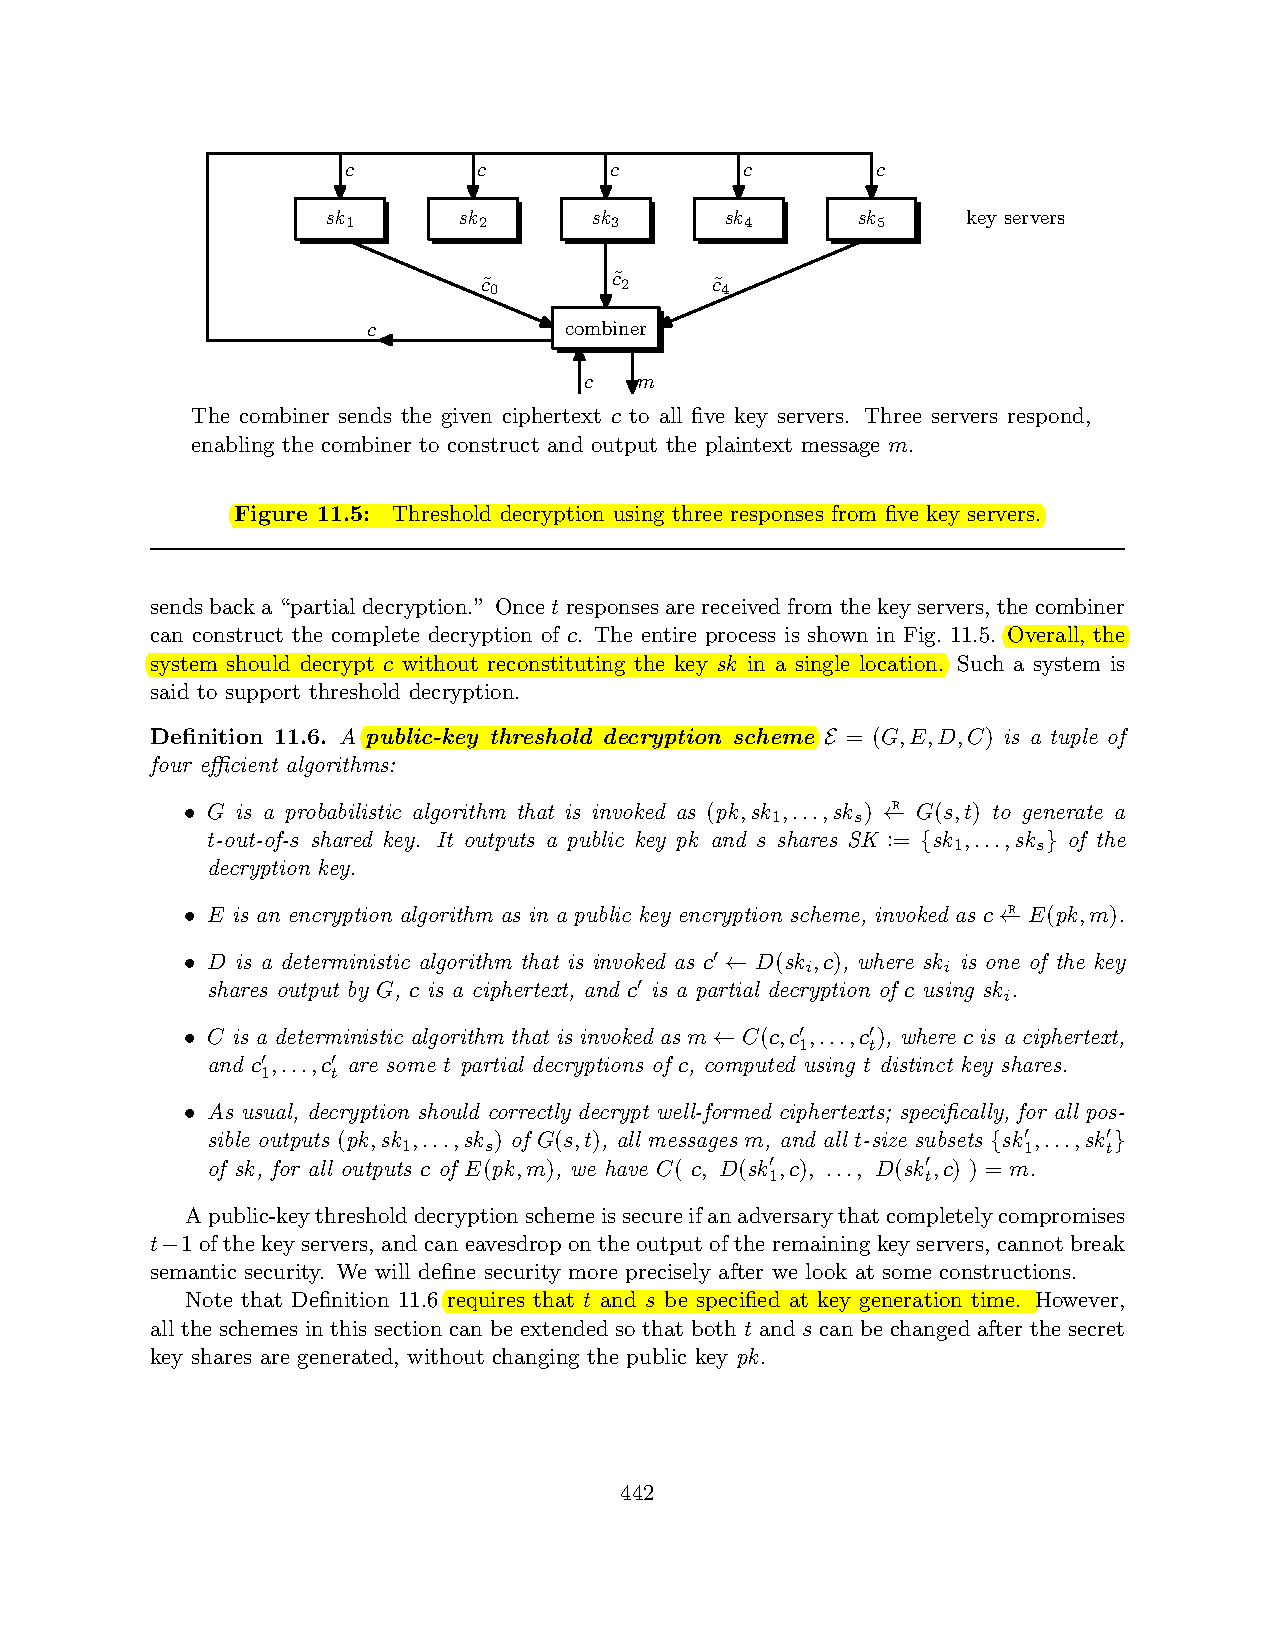
\includegraphics[clip, trim=3cm 21.2cm 3cm 2cm, width=1.00\textwidth]{img/threshold_decryption_excerpt.pdf}
    \caption{Übersicht über den Entschlüsselungsvorgang bei der Nutzung eines (3,5)-Schwellwertschemas. Entnommen aus \cite{boneh2016}.}
    \label{fig:threshold_decryption_combiner}
\end{figure}

In \cite{boneh2016} werden diese Systeme formalisiert. Ein \textit{Threshold-Public-Key-Decryption}-Schema \(\epsilon = (G, E, D, C)\) besteht aus vier Algorithmen: 

\begin{itemize}
  \item \(G(t, n, r)\) ist der Algorithmus zur Generation des öffentlichen Schlüssels \(pk\) und der \(n\) \textit{Shares} des geheimen Schlüssels \(\{sk_1, \dots, sk_n\}\). \(t\) steht für die Anzahl der zur Entschlüsselung benötigten \textit{Shares}. \(r\) ist als stellvertretend für die einfließenden Zufallswerte zu betrachten.
  
  \item \(E(pk, m, r)\) steht für den Algorithmus, der der Verschlüsselung eines Klartexts \(m\) mit dem öffentlichen Schlüssel \(pk\) dient. \(r\) dient der Vermeidung von \textit{Known-Ciphertext-Angriffen}. \todo{Vmtl.? Mehr Details...}
  
  \item \(D(sk_i, c)\) ist der Algorithmus der für einen bestimmten \textit{Share} und einen Schlüsseltext \(c\) eine partielle Entschlüsselung \(c_j'\) liefert.\todo{EZ: c' ist ungeeignet fuer die Benennung eines Entschluesselungsergebnisses, wenn du den Schluesseltext mit c bezeichnest. Wo kommt das j her?}
  
  \item \(C(c, c_1', \dots, c_t')\) ist der Algorithmus, der aus dem Schlüsseltext \(c\) und aus \(t\) durch \(D\) generierten partiellen Entschlüsselungen wieder den Klartext \(m\) liefert. Dieser Algorithmus wird auch \textit{Combiner} genannt. 
\end{itemize}

Zusätzlich wird von diesen Algorithmen die folgende Eigenschaft verlangt. Sie beschreibt die korrekte Entschlüsselung von validen Schlüsseltexten im Kontext eines Schwellwertschemas: Für alle möglichen Ergebnisse \((pk, \{sk_1, \dots, sk_n\})\) von \(G\), alle möglichen Nachrichten \(m\) und alle \(t\)-elementigen Teilmengen der \textit{Shares} \(\{sk_1', \dots, sk_t'\}\) soll für alle möglichen Schlüsseltexte \(c=E(pk, m, r)\) gelten: \(C(c, D(sk_1', c), \dots, D(sk_t', c)) = m\).

Eine Übersicht über den Entschlüsselungsvorgang ist in Abbildung \ref{fig:threshold_decryption_combiner} zu finden. Dort sind die partiellen Entschlüsselungen und der \textit{Combine}-Vorgang eines \((3,5)\)-Schwellwertschemas dargestellt. Der Algorithmus \(D\) für die partielle Entschlüsselung läuft dabei auf den einzelnen \textit{Key-Servern} ab.

In \cite{boneh2006} werden diese Algorithmen noch um einen fünften erweitert, der dazu dient, einzelne partielle Entschlüsselungen auf Validität zu überprüfen. Hierdurch können fehlerhaft handelnde \textit{Key-Server} aufgedeckt werden. Hierzu wird auch der Algorithmus \(G\) verändert, der zusätzlich einen Validierungsschlüssel \(vk\) liefert:
\begin{enumerate}
	\item \(G(t, n, r)\) liefert nun \((pk, vk, \{sk_1, \dots, sk_n\})\).
  \item[...] 
  \setcounter{enumi}{4}
	\item \(V(pk, vk, c, c_j')\) überprüft die \(j\)-te partielle Entschlüsselungen auf Validität.
\end{enumerate}

Weiterhin wird für den neuen Algorithmus eine weitere Eigenschaft verlangt. Für jeden Schlüsseltext \(c\) und \(c_j' = D(sk_i,c)\), wobei \(sk_i\) der \(i\)-te von \(G\) erstellte \textit{Share} ist, gelte: \(V(pk, vk, c, c_j')\) liefert ein valides Ergebnis.



\section{Weitere kryptographische Verfahren und Techniken}

In diesem Abschnitt werden die Grundlagen weiterer kryptographischer Verfahren und Techniken vorgestellt, die in dieser Arbeit verwendet werden.

% Aus der BA

\subsection{Hashfunktion}

Eine Hashfunktion ist eine Funktion, die eine Eingabe variabler Länge auf eine Ausgabe fester Länge (den Hashwert) abbildet.\\
In der Kryptographie werden meist kryptographisch sichere Hashfunktionen eingesetzt. Bei dieser Art von Hashfunktionen handelt es sich um Einwegfunktionen, d.h. es ist leicht, aus einer Eingabe den Hashwert zu berechnen, jedoch nicht mit vertretbarem Aufwand möglich, zu einem gegebenen Hashwert eine Eingabe zu finden, die auf diesen Wert abgebildet wird. Zusätzlich müssen die Hashfunktionen kollisionsresistent sein: Für einen gegebenen Wert ist es praktisch nicht möglich einen zweiten Wert zu finden, der den gleichen Hashwert besitzt \cite{Schneier2006}.

\subsection{Message Authentication Code}

\label{sec_mac}

Ein Message Authentication Code (MAC) ist ein Verfahren, das dazu dient, die Authentizität und die Integrität einer Nachricht sicherzustellen. Dazu wird vom Sender aus einem geheimen Schlüssel \(k\) und der Nachricht \(m\) eine Art Prüfsumme generiert und zusammen mit der Nachricht versendet. Ein Empfänger kann den MAC überprüfen, wenn er im Besitz des gleichen geheimen Schlüssels ist, und so sicher sein, dass die Nachricht nicht verändert wurde \cite{Schneier2006}.

\subsection{Hybride Kryptosysteme}

\label{sec_basics_hybrid}

Als hybrides Kryptosystem wird die Kombination von symmetrischen und asymmetrischen Kryptoverfahren zur Verschlüsselung bzw. Entschlüsselung einer Nachricht bezeichnet. Ein Schlüssel \(k_{symm}\) für die Verwendung im symmetrischen Verfahren wird zufällig erzeugt und mithilfe des öffentlichen Schlüssels eines asymmetrischen Verfahren als \(c_{public}\) verschlüsselt. Der zu verschlüsselnde Klartext \(m\) wird anschließend mithilfe des symmetrischen Verfahrens und des erzeugten Schlüssels \(k_{symm}\) als Chiffretext \(c_{symm}\) verschlüsselt. \\
Zur Entschlüsselung wird \(c_{public}\) mit dem geheimen Schlüssel des asymmetrischen Verfahrens entschlüsselt. Der hieraus erhaltene Schlüssel \(k_symm\) kann nun zur Entschlüsselung von \(c_{symm}\) genutzt werden, um \(m\) zu erhalten \cite{katz2014}.

Der Vorteil dieser Lösung beruht darin, dass Vorteile symmetrischer und asymmetrischer Verfahren kombiniert werden: Symmetrische Verfahren sind im Allgemeinen deutlich schneller als asymmetrische, die jedoch das bei symmetrischen Systemen bestehende Problem des Schlüsselaustauschs lösen.

\subsection{Authenticated Encryption Schemes}

\label{sec_basics_ae}

Symmetrische Kryptosysteme sorgen erst einmal nur für den Schutz der Vertraulichkeit einer Nachricht. Wird zusätzlich die Integrität einer Nachricht durch das System geschützt, so spricht man von einem \textit{Authenticated Encryption Scheme}. Hierdurch wird erreicht, dass Änderungen am Schlüsseltext bei der Entschlüsselung erkannt werden und der Vorgang abgebrochen werden kann.\\
Ein solches System kann durch Berechnung eines MACs zusätzlich zur Verschlüsselung erreicht werden. Alternativ dazu gibt es Schemata, die direkt auf einer Blockchiffre aufbauen \cite{boneh2016}. Ein Beispiel hierzu ist der GCM-Betriebsmodus, der in Kombination mit AES in vielen verbreiteten Protokollen wie TLS zu finden ist.


\subsection{ElGamal-Kryptosystem}

\label{sec_basics_threshold_elgamal}

Im Folgenden sei \(\mathbb{G}\) eine zyklische Gruppe der primen Ordnung \(p\) und \(g\) ein Generator dieser Gruppe. Diese Parameter können öffentlich bekannt gegeben werden. Alle folgenden Berechnungen werden in \(\mathbb{G}\) (also modulo \(p\)) ausgeführt.

Ein Teilnehmer wählt nun ein zufälliges Element \(x \in \mathbb{Z}_p\). Dies ist der private Schlüssel des Teilnehmers. Er berechnet zusätzlich seinen öffentlichen Schlüssel \(h = g^x\).\\
Um eine Nachricht \(m\), die an den Teilnehmer geschickt werden soll, zu verschlüsseln, wird zuerst ein zufälliges Element \(y \in \mathbb{Z}_p\) gewählt. Anschließend kann die Nachricht verschlüsselt als \((v, c) = (g^y, h^y \cdot m)\) versendet werden.\\
Zur Entschlüsselung berechnet der Empfänger \(k' = (v^x)^{(-1)}\) und kann die Nachricht \(m = c \cdot k'\) entschlüsseln. Dies funktioniert, da 
\[c \cdot k' = (h^y \cdot m) \cdot (v^x)^{(-1)} = g^{xy} \cdot m \cdot g^{(-yx)} = m\]
gilt.

Die Sicherheit des Verfahrens beruht auf dem Diskreten-Logarithmus-Problem. Details und Beweise hierzu sind beispielsweise in \cite{katz2014} zu finden. \todo{Erweitern, um später darauf zurückgreifen zu können}


\section{Searchable Symmetric Encryption}

\label{sec_basisc_se}

%- Searchable Symmetric encryption vs Public Key Encryption With Keyword Search
%- Hier relevant SSE

\textit{Searchable Symmetric Encryption} (SSE) ist ein Konzept , das es ermöglicht, Daten in verschlüsselter Form auf einen Server auszulagern und trotzdem Suchanfragen auf den Daten ausführen zu können. Ein allgemeines SSE-Schema besteht aus vier effizient berechenbaren Algorithmen \cite{wang2016}:

\begin{itemize}
  \item \textbf{GenerateKey}\((k)\) generiert einen geheimen Schlüssel \(K\) anhand eines (verfahrensabhängigen) Sicherheitsparameters \(k\).
  \item \textbf{BuildIndex}\((K, D)\) erstellt einen Suchwort-Index \(I\) aus dem generierten Schlüssel \(K\) und einer Dokumentenmenge \(D\).
  \item \textbf{GenerateTrapdoor}\((K, w)\) erstellt für ein spezielles Suchwort \(w\) mithilfe des Schlüssels \(K\) das Trapdoor-Element \(T_w\) für die Suche nach \(w\).
  \item \textbf{Search}\((I, T_w)\) liefert eine Menge von Dokumenten basierend auf einem Suchwort-Index \(I\) und einem Trapdoor-Element \(T_w\).
\end{itemize}

Der Besitzer der Daten erstellt sich einen Schlüssel mithilfe von \textbf{GenerateKey} und generiert durch \textbf{BuildIndex} einen Suchwort-Index für seine Dokumente. Anschließend lädt er diese Dokumente in verschlüsselter Form zusammen mit dem Index auf den Server. Möchte der Besitzer nun alle Dokumente erhalten, auf die ein spezielles Suchwort zutrifft, so erstellt er für dieses Suchwort mithilfe von \textbf{GenerateTrapdoor} ein Trapdoor-Element und sendet dieses an den Server. Dort wird nun auf dem Suchwort-Index durch \textbf{Search} die Suche nach dem Trapdoor-Element ausgeführt, die eine Menge von verschlüsselten Dokumenten liefert, auf die das Suchwort zutrifft. Diese können zurück an den Besitzer gesendet werden, der sie lokal entschlüsseln kann. 